\subsection{Traffic investigation}
\subsubsection{RF layer}
Regarding the RF layer a few messages can be seen there. As shown in the appendix \ref{app:ubertooth} the most packets seen are the NULL and POLL messages, that are keep alive messages. During the captures the Ubertooth is only looking at channel 0 on which these packets are sent.

Some other packets are decoded by the Ubertooth and contains some data, the packets over the RF layer are of a different types. The packet decoded are of type DV/3-DH1, AUX1, AFH, DM1, HV1, DH5/3-DH5. An explanation of these packet types are explained in this appendix \ref{app:types} .

The only valuable information that could be output from this data analysis is that the packets sent between the smartwatch and the phone are fragmented as they contain different LLID parameters (which specifies if the payload is the start or the continuation of a L2CAP or LMP message). The packets are also encrypted.

\subsubsection{HCI layer}
From the HCI captures, some conclusions can be drawn. Indeed, during the pairing process, some parameters are negotiated regarding the future communication between the two devices. SSP introduces IO capabilities that permits to exchanged what would be the pairing model based on the capability of the master and slave device. 
\begin{figure}[!h]
  \begin{center}
	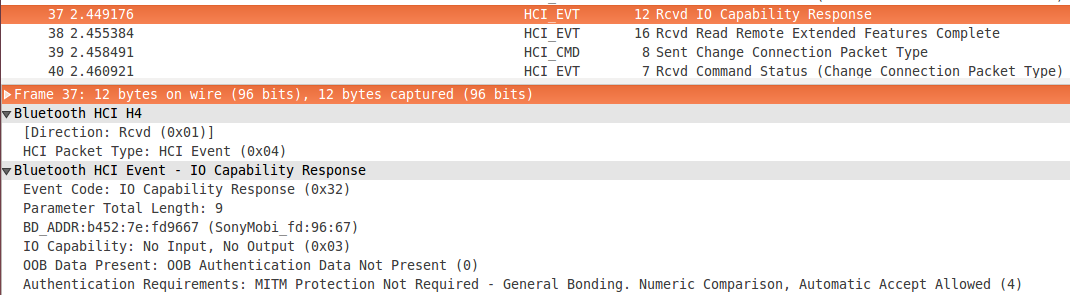
\includegraphics[width=270px]{images/IO_PARAM.png}
	\label{fig:io}
	\caption{IO capabilities found during the pairing process at the HCI layer}
  \end{center}
\end{figure}
The pairing process analysing shows that the pairing process the watch and the phone is based on JustWork mechanism. Indeed, as shown in \ref{fig:io} the Smartwatch claim not to have any input or output and that it does not have OOB authentication then the two devices agree to set up their connection with the JustWork mechanism that involves automatic accept of the numeric comparison. This mechanism is not protected from a MiTM attack.

Then the LMP parameters \ref{fig:lmp} are exchanged to choose the LMP parameters that will be used during this communication. 
\begin{figure}[!h]
  \begin{center}
	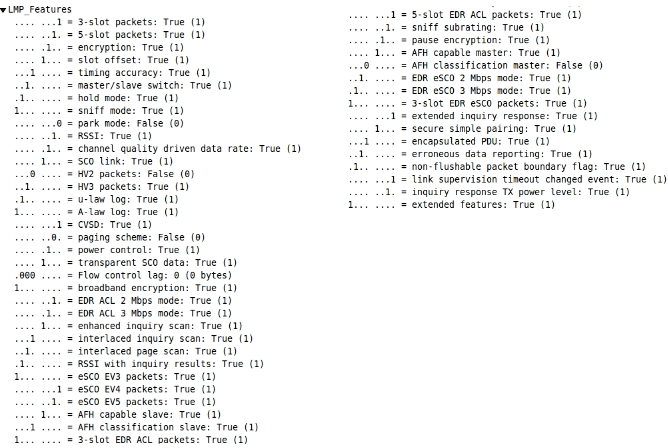
\includegraphics[width=270px]{images/LMP_PARAM.jpg}
	\label{fig:lmp}
	\caption{LMP Parameters found during the pairing process at the HCI layer}
  \end{center}
\end{figure}

From there, it is true to say that the communication is encrypted, encapsulated and uses SSP. It is even possible to retrieve the link keys used for encryption at this level. The link keys are always updated after a new pairing.

\subsubsection{Correlation of the two layers}

%Why cant we correlate the packet seen on Rf to hci? 
%Maybe we should trey to decrypt a packet using the key we found nat the hci. Just to proove that it is possible to decrypt the packets if we would have the key. ANd we would have the key maybe if the ubertooth was doing what we did.
Firstly the POLL and NULL packet are not available at the HCI layer. They are destined and processed at the link controller layer so they cannot be seen.

\textbf{The 6 other types of packets found can or cannot be correlated?}

Another thing that can be highlighted from the pairing process on the HCI, is that the master and the slave exchange information about what kind of packets are allowed during the communication. During this exchange the connection set up these packet types are disallowed. As you can see in appendix \ref{app:pairing}.  \pend


\subsection{The rogue packets}
As already mentioned, there are some packets we cannot place. These are packets that can be found by the Ubertooth, but cannot be detected by the HCI. These messages are handled in the LC see figure \ref{subsubsec:rflayer}.
Some examples are seen in appendix \ref{app:roguepackets}.
Looking at the first packet in appendix \ref{app:roguepackets} there are a few things that can be seen. The packets with data are always doubled. The reason for this is unknown. The unwhitened packet is divided in a few fields. Type, LT\_ADDR, flow, payload length and data. The first line contains some information about the packet. The most important values from this information are:
\begin{itemize} 
\item The \textbf{ch}, this is the channel in which the packet was found.
\item The \textbf{LAP}, which is the sender's lower address part.
\end{itemize}
The reason that the type has two values is that for different data rates the packet type can differ. The SW2 has no voice capabilities and knows high data transfer rate. In specifications table that can be found 308 in the last column. So the packet types will always be the latter of the two types given.
The LT\ADDR is used to determine which is used by each receiving device to determine if the packet addressed to them, but it is also used ffor internal routing.
The LLID is the (Logical Link Identifier)
To analyse the payload the authors have tried to decode these packets using the key exchanged during the pairing process.
%BUT WE FAILED/ ANALYSED HOW WE CAN DO THAT